\subsection{Overview}
As stated above, each subsystem has to accomplish its own goal. In particular, we can see AutomatedSOS and Track4Run as simple  applications for smart-devices, while Data4Help is a service provider that should implement a more complex, scalability-oriented architecture.

The figure below gives a general overview of a possible implementation of the system.

\FloatBarrier

\begin{figure}[!h]
	\centering
	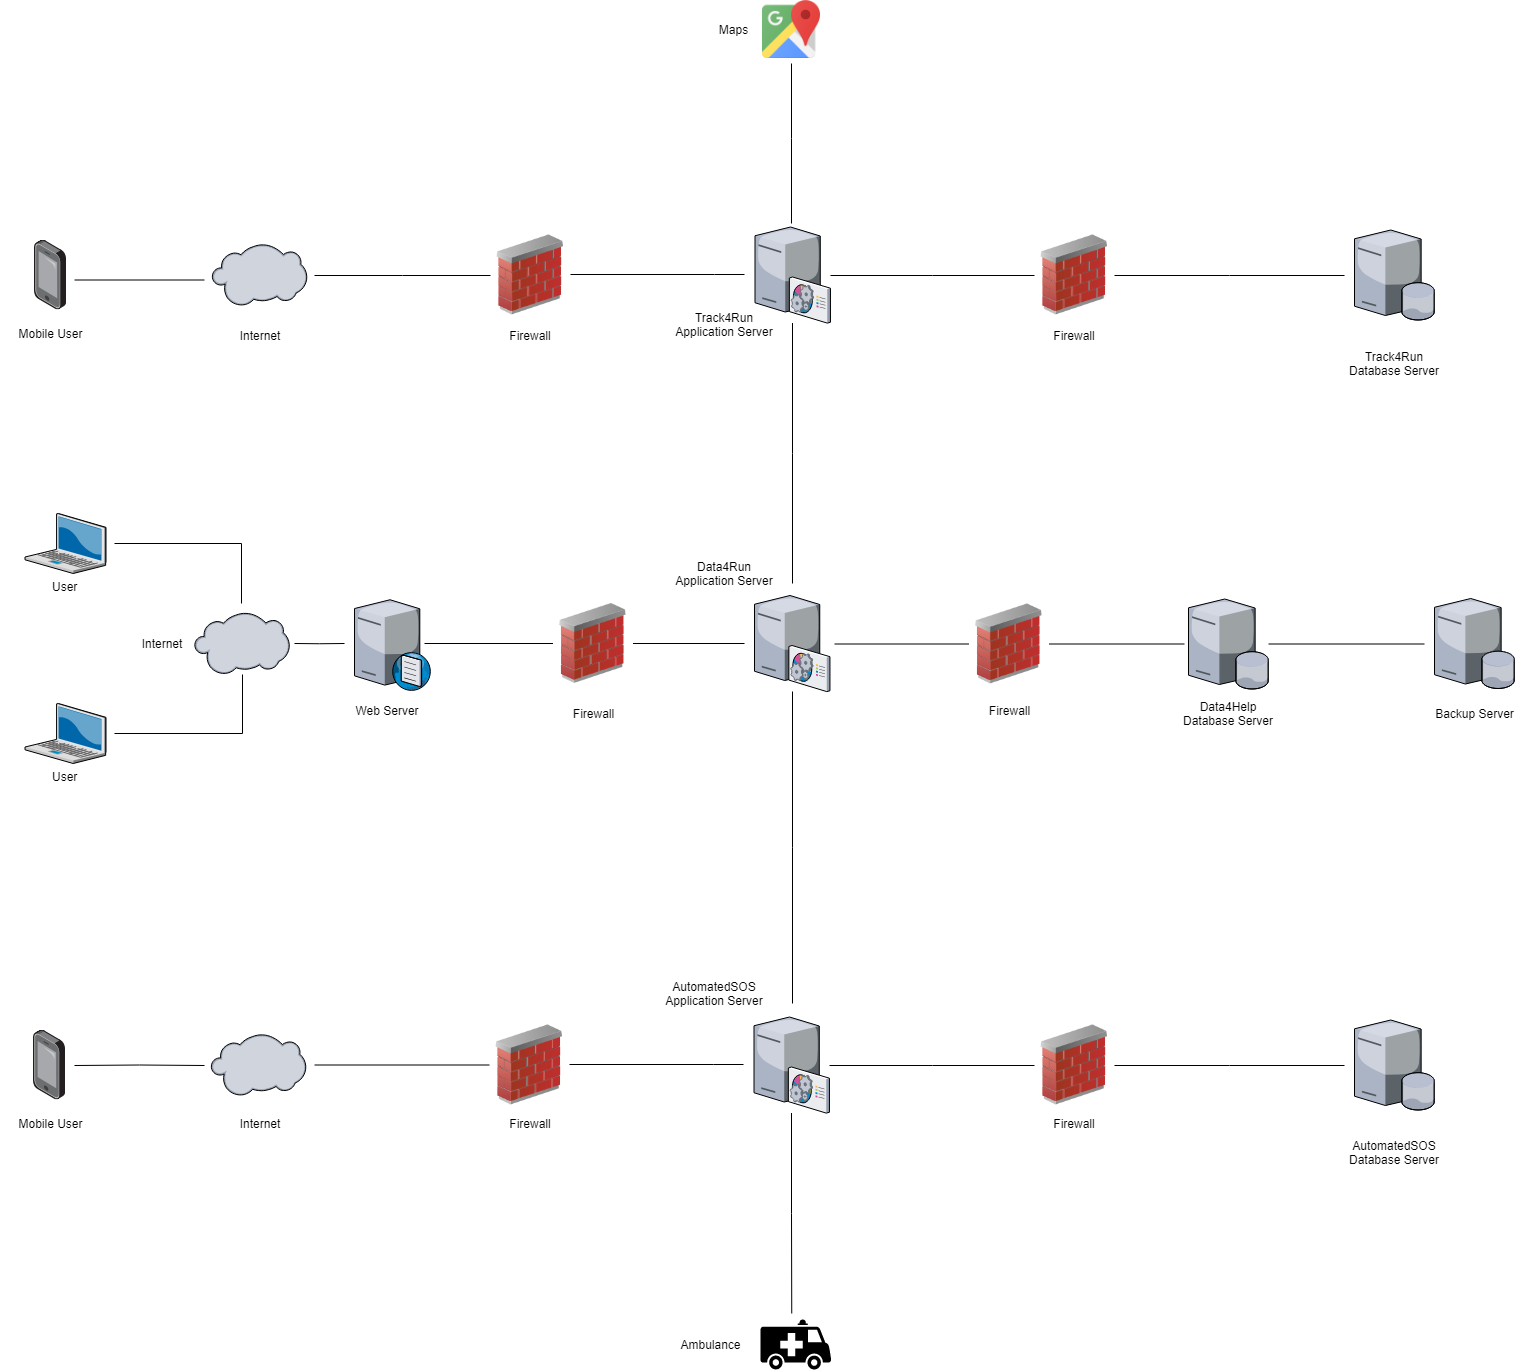
\includegraphics[width=\columnwidth]{physicalArchitectureDiagram.png}
	\caption{General Architecture}
\end{figure}


\FloatBarrier

As displayed in this figure, Data4Help subsystem's services can be accessed by many channels, including a web interface for users and APIs for data-sources and third-parties.
Since the data-sources provide real-time data from the user's devices, it is predictable that this flow of information will soon grow into a huge number of requests, so this subsystem has to be designed to quickly accomplish horizontal scaling and maintain high availability even in extreme conditions.
For this reason, a Microservice based architecture enforced with Message Queues and scalable databases should be adopted, as will be described in the following sections. Also an API Gateway is used to access all Data4Help interfaces, so to easily manage authentication and load balancing from the very first moment of any request.

AutomatedSOS and Track4Run instead are designed as three-tier applications with a thick client (i.e. smart-phone and smart-watch apps), a lightweight back-end server and a storage module. This design has been chosen because it is completely modular on one hand, since the two application's business logic is separated from Data4Help's one, but guarantees on the other hand a fast and reliable service provided by the servers, leaving the full responsibility of the presentation part to the mobile application. The separation of presentation and business logic also guarantees the maintainability of the system and good performances on mobile devices, where power consumption and CPU usage can be an issue.

\subsection{High Level Architecture}

From the component point of view, each subsystem can be divided into \textit{back-end} components, which are responsible of carrying out the business logic of the subsystem, and \textit{front-end} components, which provide a presentation layer to end users and SDKs to external developers who want to access the system's services.
Also, some external components are used to provide some of the services offered by the system.
In the following diagram, the main components and interfaces are highlighted, to give a general idea of the design of the system.
It must be noted that in this diagram components and \textit{modules} represent a set of services grouped together, and that internal interaction between modules is not shown for sake of simplicity: the complete description of all the modules and internal interfaces can be found in the following sections.

\FloatBarrier
\begin{figure}[!h]
	\centering
	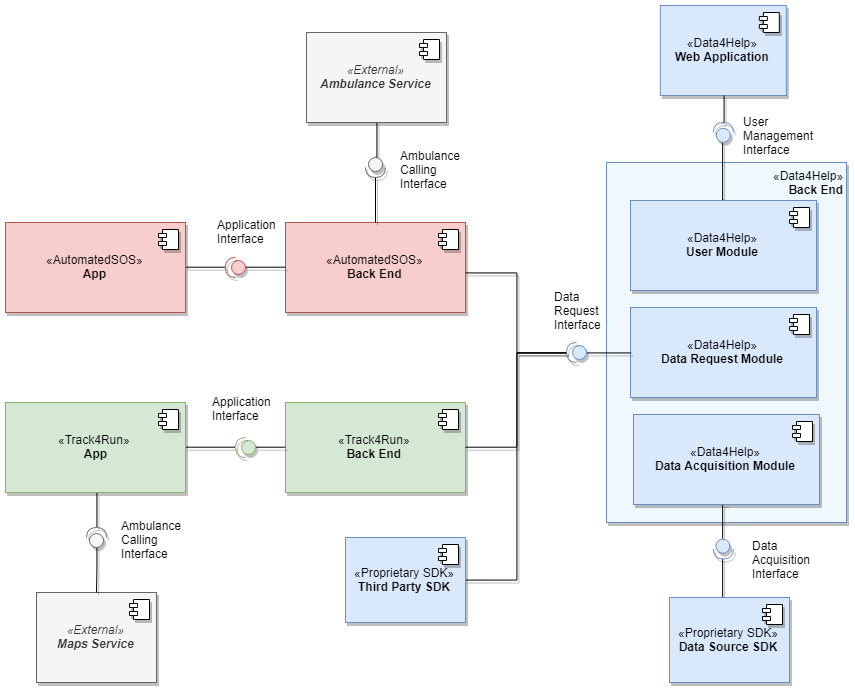
\includegraphics[width=\columnwidth]{ComponentDiagrams-Total.png}
	\caption{High Level Components}
\end{figure}
\FloatBarrier

As can be seen, the Data4Help back-end is composed of four major modules:

\begin{itemize}
	\item \textit{User Management}: provides an interface for managing the user account and configure his data-sources. This interface is exploited by a \textit{Web Application} that can be accessed via web browser.
	\item \textit{Data Acquisition}: provides the interface for collecting data from data-sources. A proprietary \textit{Data Source SDK} can be offered to external developers to integrate the use of this interface into their software and send data from external devices to Data4Help.
	\item \textit{User Management}: enables third parties to make requests on the data received by the subsystem. This interface is used by \textit{Track4Run} and \textit{AutomatedSOS} back-ends, but it can also be accessed by any other third party via the dedicated \textit{Third Party SDK} that is offered to third-party developers.
	\item \textit{Authentication}: enables the system to recognize and authenticate incoming requests and associate them to a specific User, Third Party or Data-Source.
\end{itemize}

The other two back-ends are mainly responsible of exploiting Data4Help's serviced to offer an interface to the user's Application. 

\begin{itemize}
	\item \textit{AutomatedSOS App Interface}: provides the functions to login a user, modify its threshold and monitor its health state.
	\item \textit{Track4Run App Interface}: provides the functions to login a user, create and modify a run, search runs, join a run a watch runners.
\end{itemize}

Finally there are the external services: for AutomatedSOS, an external ambulance calling interface is needed by the back-end to fulfill its goals, while in Track4Run a Maps Service such as \textit{Google Maps} should be accessed directly from the Application to minimize latency and bandwidth occupation in the communication between the client and the server.
\\

Another definition of the services offered by the system can be found in the figure below, which highlights the dependencies between the Data4Help system and its actors and provides a list of the services consumed internally and externally by the system.

\FloatBarrier
\begin{figure}[!h]
	\centering
	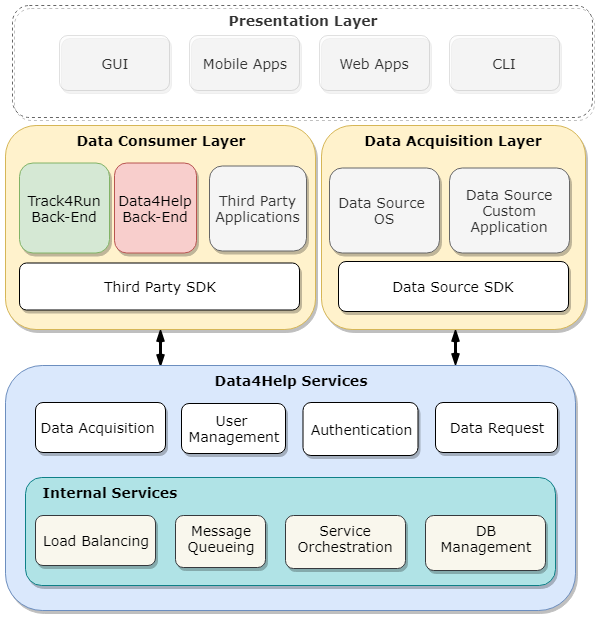
\includegraphics[width=0.8\columnwidth]{ComponentDiagrams-Layers.png}
	\caption{System Layers Architecture}
\end{figure}
\FloatBarrier

The whole system's internal and external services can be divided into five layers:
\begin{itemize}
	\item \textit{D4H Internal Services Layer}: these components are used internally by Data4Help to provide highly available services. They mainly deal with microservices management and will not be discussed in the detailed architecture, since there are many available options on the market such as Docker and Kubernetes for container management, MongoDB for data management, RabbitMQ for message queueing etc...
	
	\item \textit{D4H External Services Layer}: this layer provides the four main functionalities of Data4Help, which have been discussed in the previous part.
	
	\item \textit{Data Acquisition Layer}: also this layer is built upon Data4Help Services. It contains the SDK on which external data-source software can rely to send collected data to Data4Help.
	
	\item \textit{Data Consumer Layer}: this layer is built upon Data4Help Services and contains the SDK that can be used by third parties to make API requests, as well ad the whole AutomatedSOS and Track4Run back-ends, which are in this sense \textit{consumers} of the Data4Help services.
	
	\item \textit{Presentation Layer}: can be built upon the previous layers, in the case of AutomatedSOS and Track4Run, this layer represents the mobile application, which provides a GUI to the end user. Also data-sources and external third-parties can offer a presentation layer to their end-users.
\end{itemize}


\subsection{Component View}


\subsubsection{Data4Help}

When considering the architecture for Data4Help, the first thing to take into account is scaling and availability. The main focus of this design is that every service should be replicable in any desired number of instances without the need of changing other parts of the system. For this to be possible, the system should make use of a microservice architecture and message queues.

This said, here is a detailed view of the components of this subsystem: each service is to be considered as independently deployed in a \textit{container}, which is managed by the \textit{orchestrator}. For the sake of simplicity, only the interaction between developed components is highlighted, while the components dedicated to load balancing, orchestration and services deployment are considered to be at an underlying level (see \textit{Figure 3: System Layers Architecture} in \textit{Section 2.2}).


\FloatBarrier
\begin{figure}[!h]
	\centering
	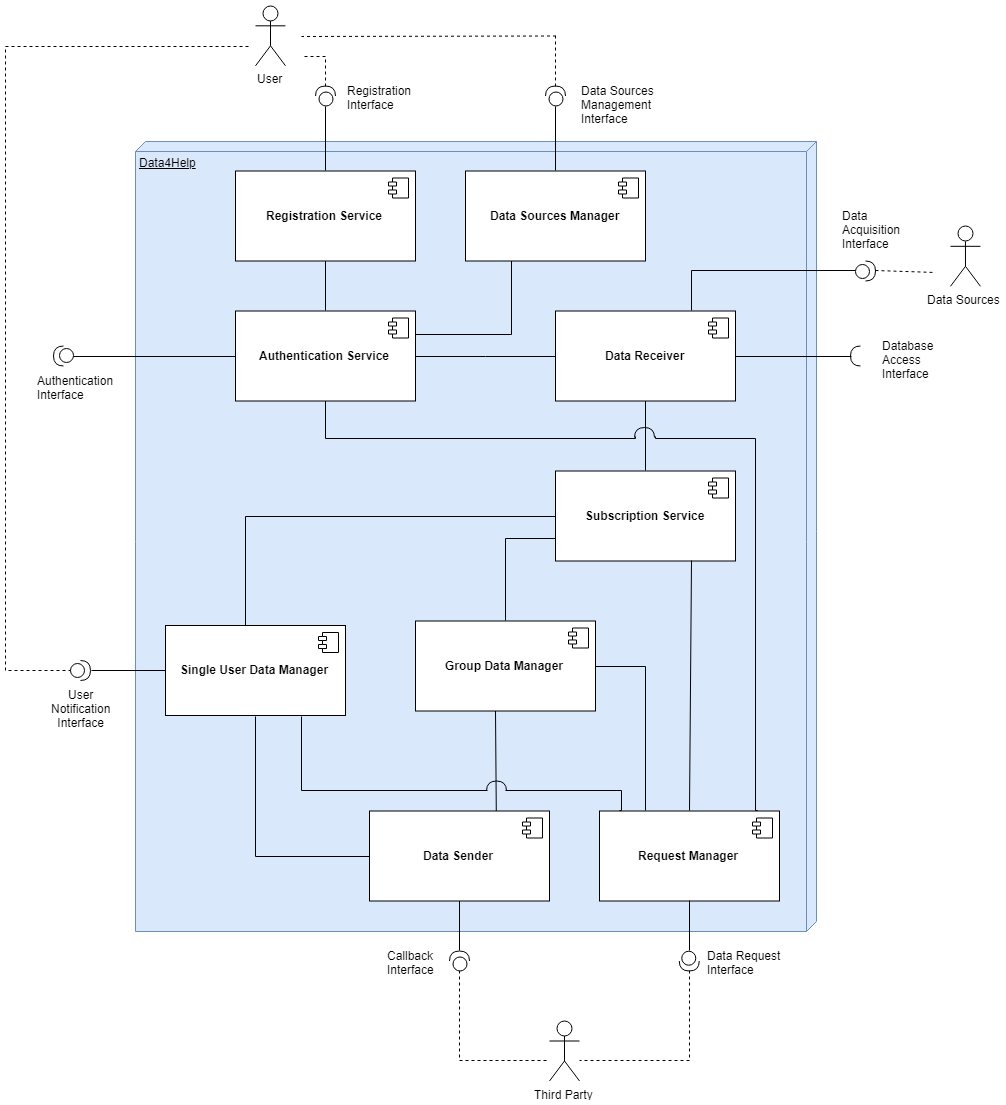
\includegraphics[width=\columnwidth]{ComponentDiagrams-Data4Help.png}
	\caption{Data4Help Components}
\end{figure}

\FloatBarrier

The internal microservices that have been identified are:
\begin{itemize}
	\item \textbf{Authentication Service}
	\item \textbf{User Service}
	\item \textbf{Receiver}
	\item \textbf{Request Manager}
	\item \textbf{Sender}
	\item \textbf{Subscription Service}
	\item \textbf{Anonymization Service}
\end{itemize}

This subsystem shall also use messaging between microservices where asyncronous communication is possible, in particular:

\begin{itemize}
	\item \textbf{New Data Queue}
	\item \textbf{New Request Queue}
	\item \textbf{Notification Queue}
	\item \textbf{Sending Queue}
\end{itemize}

All other components shall use synchronous protocols, such as RESTful APIs.

\subsubsection{AutomatedSOS}

\FloatBarrier
\begin{figure}[!h]
	\centering
	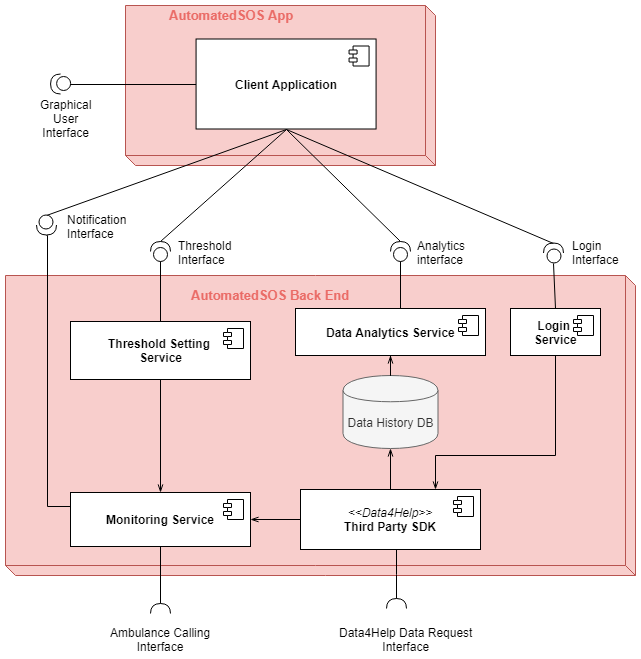
\includegraphics[width=\columnwidth]{ComponentDiagrams-AutoSOS.png}
	\caption{AutomatedSOS Components}
\end{figure}
\FloatBarrier

\begin{itemize}
	\item \textbf{Client Application:} application on user's device responsible of providing a graphical interface to the user and of interacting with the back end  services of AutomatedSOS.
	\item \textbf{Threshold Setting Service:} gives to the user the possibility to change the default threshold values of his tracked parameters and save them in the dedicated database. 
	\item \textbf{Data Analytics Service:} allows the user to check the aggregated statistics about the data collected until then with a given granularity. 
	\item \textbf{Login Service:} responsible of authenticating the user by using his Data4Help credentials using the SDK services provided by the Third Party SDK component.
	\item \textbf{Monitoring Service:} is responsible of monitoring the data coming from Data4Help and, whenever a threshold is exceeded, interacting with the external Ambulance Calling Interface which in turn will communicate to the ambulances the location of the user in danger.
	\item \textbf{Third Party SDK:} communicates with Data4Help by using his Authentication and Data Request interfaces.
\end{itemize}


\subsubsection{Track4Run}

\FloatBarrier
\begin{figure}[!h]
	\centering
	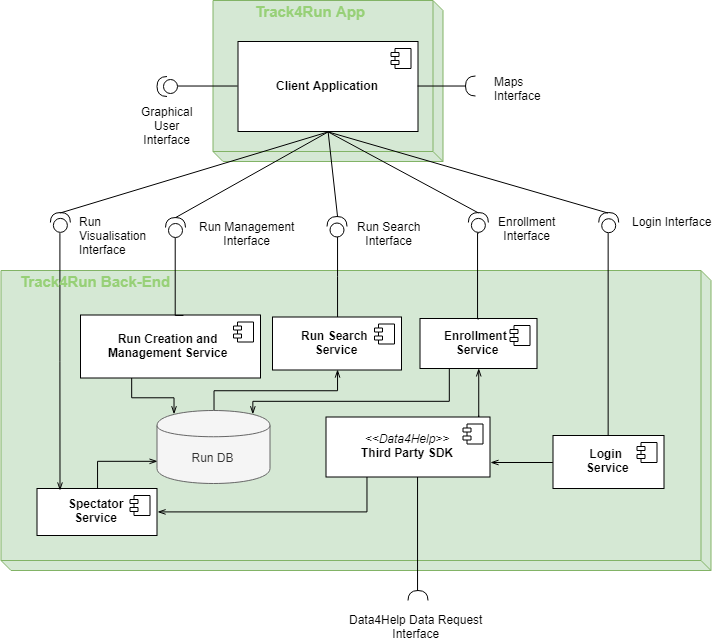
\includegraphics[width=\columnwidth]{ComponentDiagrams-Track4Run.png}
	\caption{Track4Run Components}
\end{figure}
\FloatBarrier

\begin{itemize}
	\item \textbf{Client Application:} application that runs on user's device responsible of providing a graphical interface to the user and of interacting with the back end services of Track4Run. It also interacts with an external Maps Interface in order to retrieve the maps that will be used by the application.
	\item \textbf{Run Creation and Management Service:} gives the user the possibility to create, edit and delete a run event by interacting with the Run database.
	\item \textbf{Run Search Service:} gives the user the possibility to browse all the created run events stored in the Run database.
	\item \textbf{Spectator Service:} is responsible of retrieving runners position during the run and then forwarding it to the Client Application which in turn will display the positions of the runners on a map.
	\item \textbf{Enrollment Service:} allows the user to enroll in a created run event. In this way he will be added to the list of participants.
	\item \textbf{Third Party SDK:} communicates with Data4Help by using his Authentication and Data Request interfaces.
	\item \textbf{Login Service:} responsible of authenticating the user by using his Data4Help credentials using the SDK services provided by the Third Party SDK component.
\end{itemize}


\subsection{Deployment View}

\FloatBarrier
\begin{figure}[!h]
	\centering
	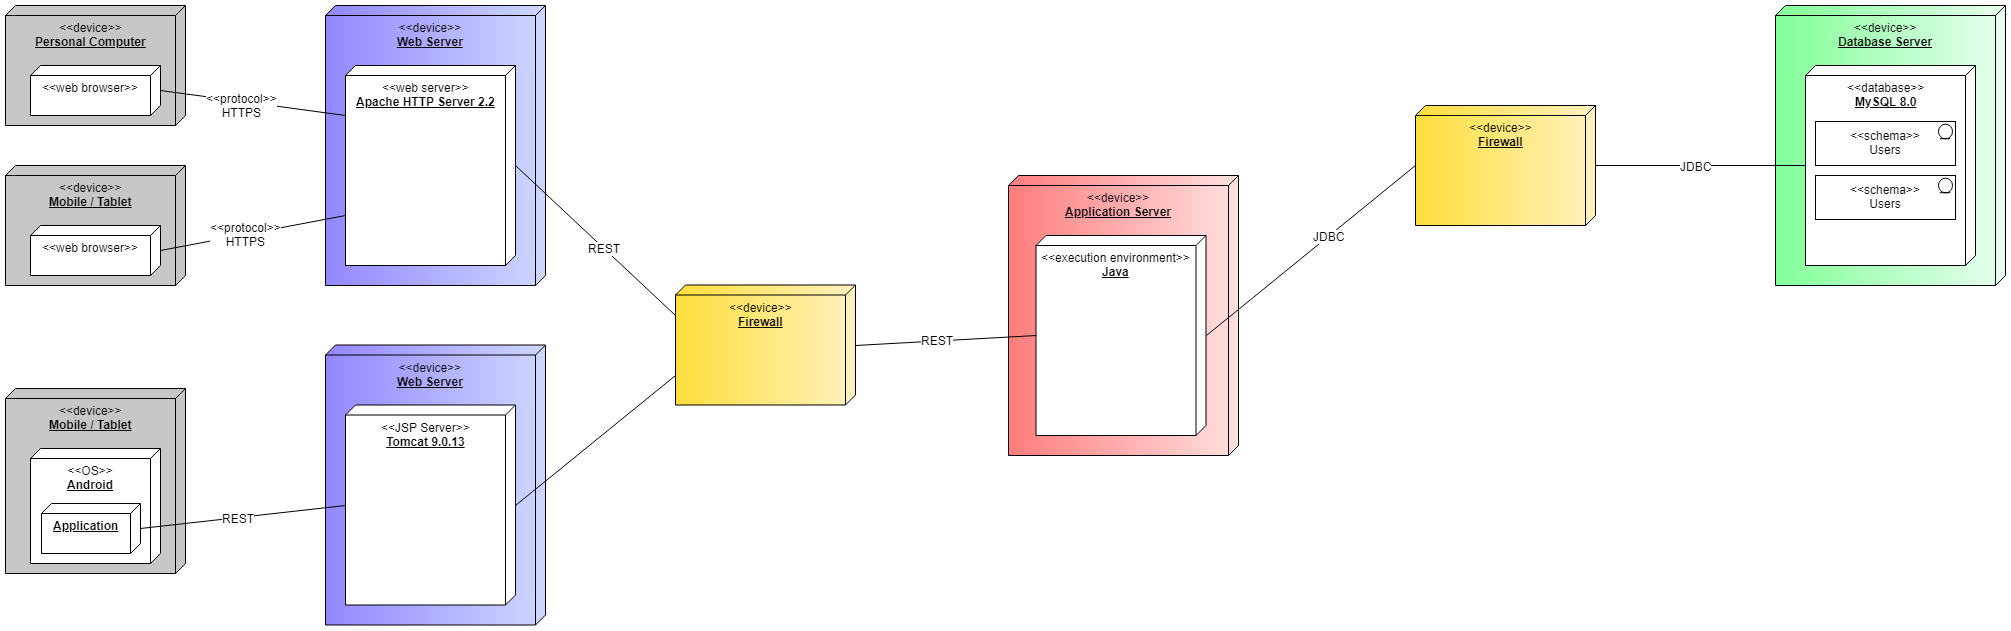
\includegraphics[angle=90, height=0.9\textheight]{deploymentDiagram.png}
	\caption{Track4Run Components}
\end{figure}
\FloatBarrier

\subsection{Runtime View}
- Auth
- One-shot req
- Subscription req
- New data arrives

\subsection{Component Interfaces}
\subsection{Selected Architectural Styles and Patterns}
- stateless
- microservice
- monolithic
- token auth
- loose coupling
- event driven and message queues
- server side service discovery
\subsection{Other Design Decisions}
- NOSQL DB
- JWT
- REST
- RabbitMQ